% generated by experiments/make_figures.py from results/db_microbench.json
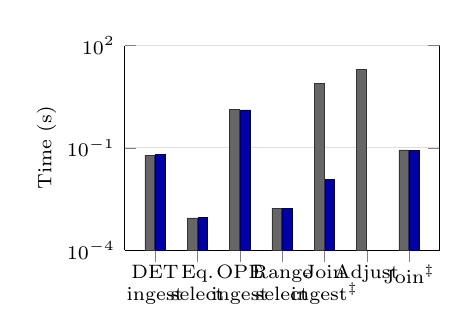
\begin{tikzpicture}
\begin{axis}[
  ybar=0.4pt, ymode=log, log origin=infty, width=0.33\textwidth, height=2.6cm,
  scale only axis,
  bar width=3.5pt, enlarge x limits=0.12, ymin=0.0001, ymax=100,
  symbolic x coords={eq_ingest,eq_select,ord_ingest,ord_select,join_ingest,join_adjust,join_run}, xtick=data,
  xticklabels={DET\\ingest,Eq.\\select,OPE\\ingest,Range\\select,Join\\ingest$^\ddagger$,Adjust,Join$^\ddagger$},
  tick label style={font=\scriptsize}, label style={font=\scriptsize},
  xticklabel style={align=center, inner sep=1pt},
  ylabel={Time (s)}, ylabel shift=-3pt, ymajorgrids, grid style={gray!25}, axis x line*=bottom,
  legend style={font=\scriptsize, draw=none, fill=none, legend columns=-1, /tikz/every even column/.append style={column sep=4pt}},
  legend image code/.code={\draw[#1] (0cm,-0.08cm) rectangle (0.22cm,0.12cm);}, legend cell align=left,
  legend to name=onionleg,
]
\addplot[fill=black!60, draw=black!80, line width=0.2pt] coordinates {(eq_ingest,0.0616215) (eq_select,0.000887615) (ord_ingest,1.34278) (ord_select,0.00169965) (join_ingest,7.70066) (join_adjust,19.8237) (join_run,0.0869211)};
\addplot[fill=blue!65!black, draw=blue!30!black, line width=0.2pt] coordinates {(eq_ingest,0.063079) (eq_select,0.000909043) (ord_ingest,1.29093) (ord_select,0.00167734) (join_ingest,0.0121706) (join_run,0.0855624)};
\legend{{CryptDB (non-PQ)},{Post-quantum}}
\end{axis}
\end{tikzpicture}\hfill
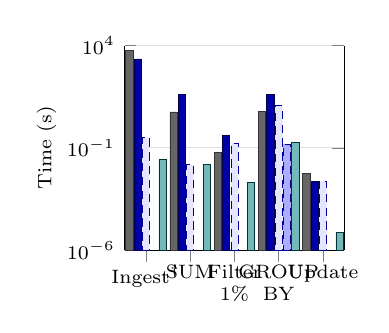
\begin{tikzpicture}
\begin{axis}[
  ybar=0.4pt, ymode=log, log origin=infty, width=0.23\textwidth, height=2.6cm,
  scale only axis,
  bar width=2.6pt, enlarge x limits=0.12, ymin=1e-06, ymax=10000,
  symbolic x coords={ingest,sum,filter,groupby,update}, xtick=data,
  xticklabels={Ingest$^\dagger$,SUM,Filter\\1\%,GROUP\\BY,Update},
  tick label style={font=\scriptsize}, label style={font=\scriptsize},
  xticklabel style={align=center, inner sep=1pt},
  ylabel={Time (s)}, ylabel shift=-3pt, ymajorgrids, grid style={gray!25}, axis x line*=bottom,
  legend style={font=\scriptsize, draw=none, fill=none, legend columns=3, /tikz/every even column/.append style={column sep=4pt}},
  legend image code/.code={\draw[#1] (0cm,-0.08cm) rectangle (0.22cm,0.12cm);}, legend cell align=left,
  legend to name=homleg,
]
\addplot[fill=black!60, draw=black!80, line width=0.2pt] coordinates {(ingest,5729.76) (sum,5.77622) (filter,0.062996) (groupby,6.06324) (update,0.00572976)};
\addplot[fill=blue!65!black, draw=blue!30!black, line width=0.2pt] coordinates {(ingest,2228.09) (sum,40.578) (filter,0.407064) (groupby,40.6597) (update,0.00222809)};
\addplot[fill=blue!10, draw=blue!60!black, densely dashed, line width=0.2pt] coordinates {(ingest,0.313039) (sum,0.0149863) (filter,0.176489) (groupby,11.659) (update,0.00238381)};
\addplot[fill=blue!32, draw=blue!50!black, densely dashed, line width=0.2pt] coordinates {(groupby,0.155546)};
\addplot[fill=teal!55, draw=teal!40!black, line width=0.2pt] coordinates {(ingest,0.0274476) (sum,0.0161504) (filter,0.0021219) (groupby,0.179039) (update,7.69479e-06)};
\addlegendimage{legend image code/.code={\draw[black, line width=1.4pt] (0cm,0.02cm) -- (0.22cm,0.02cm);}}
\legend{{Paillier, CryptDB (non-PQ)},{BFV, one value per ct.$^\dagger$ (PQ)},{BFV, packed (PQ)},{BFV, packed, client grouping (PQ)},{ASHE, AES-256 (PQ)},{Plaintext (bytes)}}
\end{axis}
\end{tikzpicture}\hfill
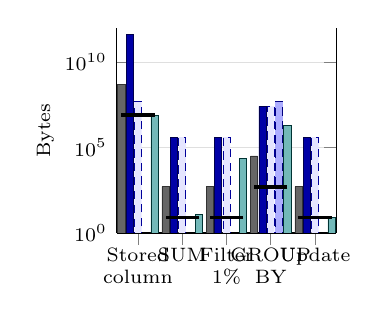
\begin{tikzpicture}
\begin{axis}[
  ybar=0.4pt, ymode=log, log origin=infty, width=0.23\textwidth, height=2.6cm,
  scale only axis,
  bar width=2.6pt, enlarge x limits=0.12, ymin=1, ymax=1e+12,
  symbolic x coords={ingest,sum,filter,groupby,update}, xtick=data,
  xticklabels={Stored\\column,SUM,Filter\\1\%,GROUP\\BY,Update},
  tick label style={font=\scriptsize}, label style={font=\scriptsize},
  xticklabel style={align=center, inner sep=1pt},
  ylabel={Bytes}, ylabel shift=-3pt, ymajorgrids, grid style={gray!25}, axis x line*=bottom,
  legend style={font=\scriptsize, draw=none, fill=none, legend columns=-1, /tikz/every even column/.append style={column sep=4pt}},
  legend image code/.code={\draw[#1] (0cm,-0.08cm) rectangle (0.22cm,0.12cm);}, legend cell align=left,
]
\addplot[fill=black!60, draw=black!80, line width=0.2pt] coordinates {(ingest,5.12e+08) (sum,512) (filter,512) (groupby,32768) (update,512)};
\addplot[fill=blue!65!black, draw=blue!30!black, line width=0.2pt] coordinates {(ingest,4.13696e+11) (sum,413696) (filter,413696) (groupby,2.64765e+07) (update,413696)};
\addplot[fill=blue!10, draw=blue!60!black, densely dashed, line width=0.2pt] coordinates {(ingest,5.08846e+07) (sum,413696) (filter,413696) (groupby,2.64765e+07) (update,413696)};
\addplot[fill=blue!32, draw=blue!50!black, densely dashed, line width=0.2pt] coordinates {(groupby,5.08846e+07)};
\addplot[fill=teal!55, draw=teal!40!black, line width=0.2pt] coordinates {(ingest,8e+06) (sum,12) (filter,22585) (groupby,2.10225e+06) (update,8)};
\addplot[only marks, mark=-, mark size=6pt, line width=1.4pt, black, bar shift=0pt, forget plot] coordinates {(ingest,8e+06) (sum,8) (filter,8) (groupby,512) (update,8)};
\end{axis}
\end{tikzpicture}

\smallskip
\pgfplotslegendfromname{onionleg}\hfill\pgfplotslegendfromname{homleg}
